\setcounter{section}{42}
\section{AVL-дерево: определение.}

\textbf{Определение.} AVL-дерево - это дерево для, которого верно условие, что если $h(v)$ - высота поддерева с корнем в $v$, то выполняется неравенство $|h(L) - h(R)| \leq 1$, где $h(L)$ и $h(R)$ - высоты поддеревьев вершины $v$. 

\textit{Аналогичное определение:} АВЛ-дерево — сбалансированное по высоте двоичное дерево поиска: для каждой его вершины высота её двух поддеревьев различается не более чем на $1$.

\setcounter{section}{43}
\section{Минимальное количество вершин $S(k)$ в AVL-дереве высоты $k$. Оценка высоты AVL-дерева на $n$ вершинах.}

\textbf{Утверждение.} Пусть $S(k)$ минимальное количество вершин в AVL-дереве высоты $k$. Тогда $S(k) = F(k + 1) - 1$.

\par $\blacktriangle$  Докажем по индукции. Для $k = 0: S(k) = 0 = F(1) - 1$. Для $k = 1: S(k) = 1 = F(2) - 1$. Для остальных значений $k = n > 1: S(n) = S(n-1) + S(n-2) + 1$, так как хотя одно поддерево корня дерева высоты $n$ должно иметь высоту $n-1$, в силу свойства дерева второе поддерево может иметь минимальную высоту $n-2$, то
$$S(n) = S(n-1) + S(n-2) + 1 = F(n) - 1 + F(n - 1) - 1 + 1 = F(n + 1) - 1 \quad \blacksquare$$

\textbf{Утверждение.} Высота AVL-дерева на $n$ вершинах равна $O(log(n))$.

\par $\blacktriangle$ В предыдущем утверждении доказывалось, что дерево высотой $h$ содержит не менее $F(h + 1) - 1$ вершин. То есть ответом на эту задачу будет максимальное $h$, такое что $S(h) = (F(h + 1) - 1) \leq n$. Так как $F_h = \Omega(\phi^h), \phi = \frac{\sqrt{5}+1}{2}$ (Из курса ОКТЧ: $F_h = \frac{1}{\sqrt(5)} \cdot \left(\frac{\sqrt{5}+1}{2}\right)^h - \frac{1}{\sqrt(5)} \cdot \left(\frac{\sqrt{5}-1}{2}\right)^h$. При $n \rightarrow \infty: F_h \rightarrow \left(\frac{\sqrt{5}+1}{2}\right)^h$), то $n \geq c_1 \phi^h$. Логарифмируя по основанию $\phi$ получим: $\log_{\phi} n c_2 \geq h$. Таким образом, получаем, что высота AVL-дерева из $n$ вершин $O(\log(n)). \quad \blacksquare$

\setcounter{section}{44}
\section{Устранение дисбаланса в AVL-дереве для случая $\delta(a) = -2$.}

Величина $\delta(a)$ обозначает разность между высотой левого и правого поддерева вершины $a$.

\textbf{Задача.} Необходимо устранить дисбаланс в дереве. $\delta(a) = -2$. Считаем, что дистбаланс присутствует только в корневой вершине. (Иначе для начала перебалансируем поддеревья корня).

\begin{figure}[h]
\begin{center}
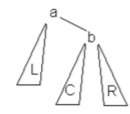
\includegraphics[width=0.2\linewidth]{images/43-46_avl_rotate}
\label{fig:mpr}
\end{center}
\end{figure}

Для разных случаях необходимо осуществить разные вращения. Малое левое вращение, если $\delta(b) = 0$ или $-1$, большое левое вращение, если $\delta(b) = 1$. Доказательство, того что эти вращения решают задачу - простое. Необходимо расписать высоты поддеревьев при заданных $\delta(a)$ и $\delta(b)$ и после вращения проверить их высоту на соотвествтвие условиям AVL-дерева. 

\subsubsection*{Малое левое вращение ($\delta(b) = -1$ или $0$)} 

\begin{figure}[h]
\begin{center}
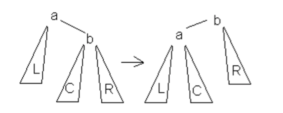
\includegraphics[width=0.4\linewidth]{images/43-46_avl_minrotate}
\label{fig:mpr}
\end{center}
\end{figure}

\subsubsection*{Большое левое вращение ($\delta(b) = 1$)}

\begin{figure}[h]
\begin{center}
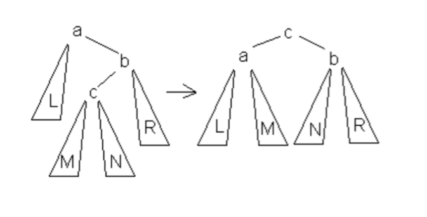
\includegraphics[width=0.4\linewidth]{images/43-46_avl_maxrotate}
\label{fig:mpr}
\end{center}
\end{figure}

\textit{Ассимптотика.} Вращения работают за $O(1)$.

\textbf{Замечение.} Если $\delta(a) = 2$, то необходимо произвести симметричные вращения: малое правое, большое правое.

\setcounter{section}{45}
\section{Реализация операций insert и erase.}

\subsubsection*{Вставка элемента.}

Необходимо добавить вершину со значением $x$. 

\textbf{Алгоритм.} 

1. Вставляем элемент как в обычном двоичном дереве.

Вершина со значением $x$ добавлена, как лист. Балланс в дереве мог нарушиться только в вершинах, которые находятся по пути от корня до добавленной вершины.

2. Поднимаемся от вершины к корню. Проверяем сбалансированность. Если разность высот поддеревьев равна 2 – выполняем нужное вращение. (Считаем, что разность высот поддеревьев не может стать больше 2. Это не просили доказывать, но проверит факт просто. Нужно посмотреть, как менятся балланс в дереве при вращении, добавлении, удалении)

\textit{Ассимптотика.} Добавление за вершины как лист: $O(log(n))$. Так как высота AVL-дерева $O(log(n))$, а вращение происходит за $O(1)$, то суммарное время добавление элемента в дерево $O(log(n))$. 

\subsubsection*{Удаление элемента.}

Необходимо удалить вершину со значением $x$. 

\textbf{Алгоритм.} 

1. Удаляем элемент как в двоичном дереве поиска

Балланс в дереве мог нарушиться только в вершинах, которые находятся по пути от корня до удалённой вершины.

2. Поднимаемся от места удалённой вершины к корню. (в и по вершине, которая встало на место удалённой. (если такая есть)) Проверяем сбалансированность. Если разность высот поддеревьев равна 2 – выполняем нужное вращение.

\textit{Ассимптотика.} Нахождение и удаление вершины из дерева: $O(log(n))$. Так как высота AVL-дерева $O(log(n))$, а вращение происходит за $O(1)$, то суммарное время удаления элемента в дереве $O(log(n))$. 